% Stay on Task: mid submission report (condensed). Build with: sh compile.sh
\documentclass[10pt,a4paper]{article}
\usepackage[T1]{fontenc}
\usepackage[utf8]{inputenc}
\usepackage{tgtermes}
\usepackage[scale=0.9]{tgheros}
\usepackage[scale=0.88]{tgcursor}
\usepackage{microtype}
\usepackage[a4paper,top=20mm,bottom=19mm,left=19mm,right=19mm,headheight=13pt]{geometry}
\usepackage[table]{xcolor}
\usepackage{graphicx,booktabs,tabularx,array,enumitem,float,amsmath,fancyhdr,lastpage,titlesec,needspace}
\usepackage[font=small,labelfont=bf,labelsep=period,skip=3pt]{caption}
\usepackage{xltabular}
\usepackage[hidelinks]{hyperref}

\definecolor{head}{gray}{0.12}
\definecolor{sub}{gray}{0.35}
\definecolor{rule}{gray}{0.55}
\definecolor{shade}{gray}{0.95}
\definecolor{rowshade}{gray}{0.955}
\definecolor{accent}{HTML}{2F5D8A}
\hypersetup{colorlinks=true,linkcolor=accent,urlcolor=accent}

\titleformat{\section}{\needspace{8\baselineskip}\sffamily\large\bfseries\color{accent}}{\thesection}{0.6em}{}[{\color{rule}\titlerule[0.5pt]}]
\titleformat{\subsection}{\needspace{5\baselineskip}\sffamily\normalsize\bfseries\color{head}}{\thesubsection}{0.6em}{}
\titlespacing*{\section}{0pt}{10pt}{4pt}
\titlespacing*{\subsection}{0pt}{6pt}{2pt}

\pagestyle{fancy}
\fancyhf{}
\fancyhead[L]{\small\sffamily\color{sub}Stay on Task: mid submission report}
\fancyhead[R]{\small\sffamily\color{sub}LMA Group Project 2026}
\fancyfoot[C]{\small\sffamily\color{sub}\thepage\ of \pageref{LastPage}}
\renewcommand{\headrulewidth}{0.3pt}
\fancypagestyle{plain}{\fancyhf{}\renewcommand{\headrulewidth}{0pt}\fancyfoot[C]{\small\sffamily\color{sub}\thepage\ of \pageref{LastPage}}}

\setlist{itemsep=1pt,topsep=2pt,parsep=0pt,leftmargin=13pt}
\setlength{\parindent}{0pt}
\setlength{\parskip}{4pt}
\renewcommand{\arraystretch}{1.15}
\newcolumntype{Y}{>{\raggedright\arraybackslash}X}
\newcolumntype{P}[1]{>{\raggedright\arraybackslash}p{#1}}
\newcommand{\tablestyle}{\footnotesize\rowcolors{2}{rowshade}{white}}
\newcommand{\code}[1]{\texttt{#1}}
\newcommand{\done}{\textbf{Done.}}
\newcommand{\run}{\textbf{In progress.}}
\newcommand{\plan}{\textbf{Planned.}}

\begin{document}

\thispagestyle{plain}
\begin{center}
{\color{rule}\rule{\linewidth}{1.2pt}}\\[4pt]
{\small\sffamily\color{sub}LMA Group Project 2026 \enspace\textperiodcentered\enspace Mid submission report \enspace\textperiodcentered\enspace 31 October 2026}\\[5pt]
{\sffamily\LARGE\bfseries\color{head} Stay on Task: can a small classifier\\[1pt] correct local agents' drift?}\\[7pt]
\begin{tabular}{cccc}
\textbf{Shuban Biswas} & \textbf{Ch Pavan Harshit} & \textbf{Swayam Goyal} & \textbf{Aaditya Sharma}\\
{\footnotesize 2024111017} & {\footnotesize 2025701057} & {\footnotesize 2024111012} & {\footnotesize 2019113009}
\end{tabular}\\[4pt]
{\footnotesize Code, data and results: \url{https://github.com/ch-pavan/lma-grp-project}}\\[2pt]
{\color{rule}\rule{\linewidth}{0.5pt}}
\end{center}

\section{Summary}
Small local agents drift, make up values and claim work they did not do. We test whether a finetuned 0.4B classifier (Laya) judges each step better than a 9B SLM judge, at a fraction of the cost. The research question, hypothesis and falsification rule are those of the revised proposal.

\textbf{Status.} The harness, datasets, baselines, annotation pipeline and first Laya results are done on validation. Test passes, test labels and the primary metric on test are not started. Every validation result is a pilot used for tuning. The claim will rest on the held out test set.

\textbf{Findings so far.}
\begin{itemize}
  \item \textbf{Step check.} On the replay step labels the head was trained on, finetuned Laya ranks bad tool calls better than the SLM judge (AUROC 0.91 against 0.61 for the judge's yes/no answers). That judge used the weaker annotator prompt. With its harness prompt and the LLM annotators' labels, Laya's F1 lead on off track tool calls is +7 to +9 points, and every interval includes zero. Three reruns on Ada put the AUROC at 0.87 $\pm$ 0.01 (0.91 is the best run), and one of the three seeds falls below the judge on off track F1, so the lead is not yet reliable. Retraining without the oracle ``breaks task'' label leaves agreement with the annotators unchanged.
  \item \textbf{Done check.} Laya's AUROC is 0.79 against 0.53 as is. F1 is 0.53 at a threshold chosen by cross validation on train (0.56) and at 0.5, against 0.41 for the SLM judge. The earlier dev threshold, from 8 dev scenarios, gave 0.36 and is dropped.
  \item \textbf{Plain rules.} On the same labels Laya beats them on both classes of the primary metric (primary F1 0.18 to 0.19 against 0.06 to 0.07; no paired interval yet). On made up values, which Laya does not output, the rules score F1 0.44 to 0.52.
  \item \textbf{Primary metric on validation.} Laya minus the SLM judge is $-$1.0 to +2.0 F1, intervals include zero. It is not met on validation. Only 6 to 15 false claims exist there and Laya has no false claim head yet, so the false claim half cannot be measured yet.
  \item \textbf{Task accuracy.} No deployable judge differs from no judge beyond noise. Rollback plus the done check helped with the oracle ceiling on Qwen3.5 4B (+9.2 [+2.5, +15.8]) and was borderline on Qwen3 8B (+5.8 [0.0, +12.5]).
  \item \textbf{Labels.} Two LLM annotators label all validation steps. After one guide rewrite their agreement with our human check is kappa 0.84 and 0.71 on a fresh sample. 0.71 is in the proposal's ``label more steps'' band, not a pass.
\end{itemize}

\begin{table}[H]
\centering\tablestyle
\caption{Where each required part of the mid submission is.}\label{tab:required}
\begin{tabularx}{\linewidth}{P{0.3\linewidth}Y}
\toprule
Progress & Sections~\ref{sec:progress} and \ref{sec:changes} \\
Datasets & Section~\ref{sec:datasets} \\
Baseline experiments & Section~\ref{sec:baselines} \\
Ablations & Section~\ref{sec:ablations} \\
Results & Sections~\ref{sec:baselines}, \ref{sec:laya} and \ref{sec:annot} \\
Challenges and mitigation & Section~\ref{sec:challenges} \\
Timeline to the final submission & Section~\ref{sec:timeline} \\
Updated GitHub with all the code & Section~\ref{sec:repo} \\
\bottomrule
\end{tabularx}
\end{table}

\section{Team}
\begin{table}[H]
\centering\tablestyle
\caption{Main work of each member. All four wrote and revised the proposal.}\label{tab:roles}
\begin{tabularx}{\linewidth}{P{0.16\linewidth}Y}
\toprule
\textbf{Shuban Biswas} & Harness and replay oracle. Qwen3 8B baselines on BFCL test and AgentDojo, Qwen3 8B and Qwen3.5 4B validation runs, correction action study, offline scorer for off the shelf judges and plain rules, blind second pass on contested check steps. \\
\textbf{Ch Pavan Harshit} & Qwen3.5 9B agent runs on Turing, LLM annotation runs, Laya finetuning of both heads, live checks and primary metric analysis, referee of the human check. \\
\textbf{Swayam Goyal} & Human check of the LLM annotations (with Aaditya), annotation guide v3, fresh check sample, Gate 1 counts, Phase 3 reruns of both heads on Ada and their scorers, report. \\
\textbf{Aaditya Sharma} & Human check of the LLM annotations (with Swayam), review of disagreements by error type. \\
\bottomrule
\end{tabularx}
\end{table}

\section{Approach}\label{sec:approach}
For each user turn a planner writes a short plan and a doer makes tool calls with Qwen3.5 9B (4 bit AWQ, reasoning off, vLLM). A judge checks each step before it runs. Laya answers typed questions with one forward pass: a step head on every tool call (is this step bad: off track, an unneeded irreversible call or a made up value on an irreversible call) and a done head at every turn end (is the request finished). The SLM judge baseline is the same 9B model with reasoning on, given the same state and guide. A bad step is rolled back and resampled, at most twice. A ``not done'' answer drops the closing message and tells the agent part of the request may be unfinished, at most twice per turn.

\begin{figure}[H]
\centering
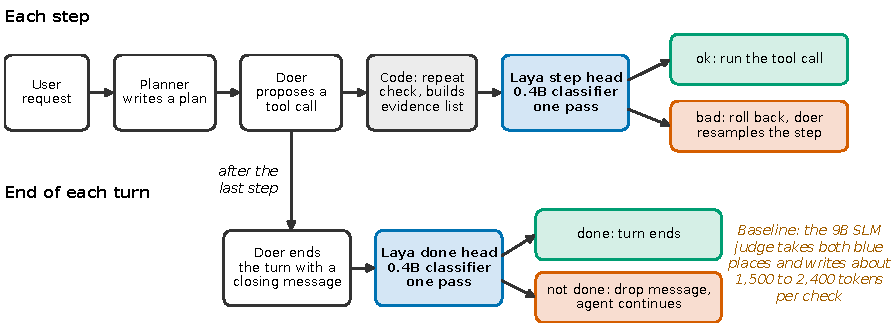
\includegraphics[width=0.93\linewidth]{figs/fig1_system.pdf}
\caption{System. The blue boxes are the two Laya checks. In the baseline the 9B SLM judge sits in both places and reasons before each answer.}\label{fig:system}
\end{figure}

\section{Progress against the proposal}\label{sec:progress}
{\tablestyle
\begin{xltabular}{\linewidth}{P{0.37\linewidth}Y}
\caption{Status of each item of the revised proposal (\code{proposal/proposal.md}).}\label{tab:progress}\\
\toprule
\textbf{Item} & \textbf{Status} \\
\midrule
\endfirsthead
\toprule
\textbf{Item} & \textbf{Status} \\
\midrule
\endhead
Harness: planner, doer, judge, rollback, done check & \done{} Gold replay passes 755 of 756 BFCL tasks and 97 of 97 AgentDojo tasks. \\
BFCL multi turn, cleaned and split, empty turn check & \done{} 74 train, 15 validation, 100 test scenarios, 11 dropped. \\
AgentDojo benign tasks (outside check) & \done{} Qwen3 8B agent, 97 tasks, 3 runs. To be rerun with the 9B. \\
Natural runs for training & \done{} 9B: 888 train tasks and 120 validation tasks. Recorded Qwen3 8B steps (356 tasks) stand in for the planned 4B pass. \\
Baselines: no judge, rules, SLM judge, Laya as is, Granite Guardian & \done{} On test with Qwen3 8B as agent and judge. Laya as is stopped at 133 runs and Granite Guardian ran as a 20 task pilot, both because they block most steps. \plan{} Rerun on the 9B for the task claim. \\
Offline judges (Kev, LettuceDetect, Laya as is) & \done{} On 1,772 validation steps. \plan{} Granite Guardian, Gemma 4 12B reference (stretch). \\
Finetuned Laya & \done{} Step head and done head. \plan{} A typed head that separates false claim from missing action. \\
LLM annotation, two annotators & \done{} All 1,772 validation steps with guide v2. Guide v3 only on the 200 checked steps. \\
Human check of the annotations & \done{} 200 steps, guide rewritten once. \plan{} 100 more steps from the test runs. \\
Step head without the oracle ``breaks task'' label; done head threshold by grouped cross validation & \done{} On Ada, 3 seeds per variant and 5 folds (Table~\ref{tab:phase3}). \\
Gate 1: 300 training examples per class & Not met. Pooled 9B and 8B steps: off track 310 and false claim 372 reach it, unneeded irreversible 217 and made up values at most 143 do not. \\
Test passes, test labels, primary metric on test & \plan{} Section~\ref{sec:timeline}. \\
Laya alone and the full system online on test & \plan{} One pass per system. \\
Escalation to the SLM judge, calibration, AgentProcessBench, AgentHallu & \plan{} Stretch, after the items above. \\
\bottomrule
\end{xltabular}}

\section{Datasets}\label{sec:datasets}
\begin{table}[H]
\centering\tablestyle
\caption{Task sets and recorded runs.}\label{tab:data}
\begin{tabularx}{\linewidth}{P{0.2\linewidth}Y}
\toprule
\textbf{BFCL v4 multi turn} & 200 scenarios in 4 versions (base, missing parameter, missing function, long context), 8 simulated apps. Cleaned: 11 unsound scenarios dropped. Split by scenario into 74 train, 15 validation and 100 test. Pass means BFCL's state checker plus our empty turn check (any state change on a turn whose correct answer is to call nothing fails). \\
\textbf{AgentDojo benign} & 97 user tasks (workspace, travel, banking, Slack), no injections, the suite's own utility check. Outside check only, never used for training or tuning. \\
\textbf{Qwen3.5 9B runs} & Validation 120 tasks (1,277 calls, 495 turn ends). Train 888 tasks (8,806 calls, 3,737 turn ends). \\
\textbf{Qwen3 8B runs} & 356 tasks on train and validation scenarios (3,824 steps) plus 3,635 gold replay steps. \\
\bottomrule
\end{tabularx}
\end{table}

\textbf{Labels.} A replay oracle labels every step automatically: after each call it replays the turn's reference calls as every possible ending, and the first call after which none passes is off track. Class balance on the 9B runs, validation and train: off track 63 of 1,277 and 221 of 8,806 calls; false claim 50 of 495 and 281 of 3,737 closing messages; turn not done 111 of 495 and 672 of 3,737. We report per class F1, precision, recall and AUROC and train with balanced class weights.

\textbf{LLM annotators.} Annotator A is DeepSeek V4.1 Flash and Annotator B is GLM 5.3 Flash. They label every validation step from a written guide without seeing the oracle labels or the BFCL verdict. Swayam and Aaditya checked these labels by hand on 200 steps and Pavan refereed (Section~\ref{sec:annot}).

\section{Baseline experiments}\label{sec:baselines}
\textbf{Systems.} S1 no judge. S2 plain rules (a value without evidence is made up, a success word without a successful call is a false claim, a call outside the plan is drift, every irreversible call asks the user). S3 SLM judge with reasoning on. S4a Laya as is. S4b Granite Guardian 3.2 3B A800M. Oracle: flags exactly the steps the replay oracle marks, a ceiling that cannot be deployed. Intervals are 95\% bootstrap over scenarios, paired for differences.

\subsection{Agent model}\label{sec:agent}
\begin{figure}[H]
\centering
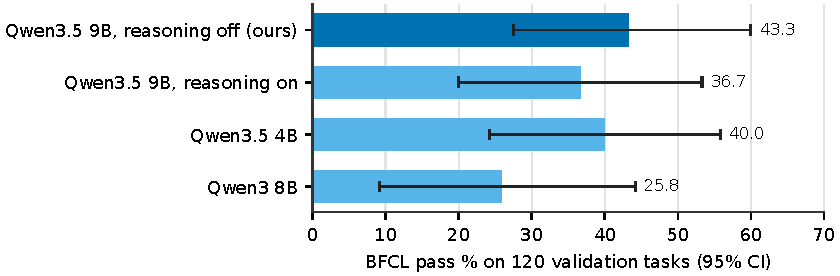
\includegraphics[width=0.55\linewidth]{figs/fig2_agents.pdf}
\caption{Agent models on the same 120 validation tasks. Qwen3.5 9B with reasoning off is our agent.}\label{fig:agents}
\end{figure}
Qwen3.5 4B passes 40.0\% against 25.8\% for Qwen3 8B, so the model generation matters more than size. The 9B passes 43.3\% on validation and 52.7\% [44.8, 60.5] on train. Reasoning on is 6.6 points lower and 2.5 times slower. About half of the 9B's failed validation tasks are unfinished turns (stopped early 26.5\%, claimed done 17.6\%, asked needlessly 8.8\%) and half are bad steps (wrong step 23.5\%, acted instead of asking 22.1\%). A judge of the proposed step cannot see an omission, which is why we added the done check.

\subsection{Online judges on the test set}\label{sec:online}
\begin{table}[H]
\centering\tablestyle
\caption{BFCL test, Qwen3 8B agent, 100 scenarios $\times$ 4 versions $\times$ 3 runs.}\label{tab:test}
\begin{tabularx}{\linewidth}{Yrlllr}
\toprule
\textbf{System} & \textbf{Runs} & \textbf{Pass \% [95\% CI]} & \textbf{vs S1 [95\% CI]} & \textbf{s / task} & \textbf{Judge tok.} \\
\midrule
S1 no judge & 1,200 & 15.9 [11.7, 20.5] & & 93 & 0 \\
S2 plain rules & 1,200 & 7.6 [4.4, 11.2] & $-$8.3 [$-$11.8, $-$5.2] & 108 & 0 \\
S3 SLM judge (Qwen3 8B) & 1,200 & 17.4 [12.8, 22.3] & +1.5 [$-$0.6, +3.8] & 202 & 11.8k \\
S4a Laya as is & 133 stopped & 0 (upper bound 2.2) & & 336 & \\
S4b Granite Guardian & 20 task pilot & 0 & & & \\
\bottomrule
\end{tabularx}
\end{table}

\begin{figure}[H]
\centering
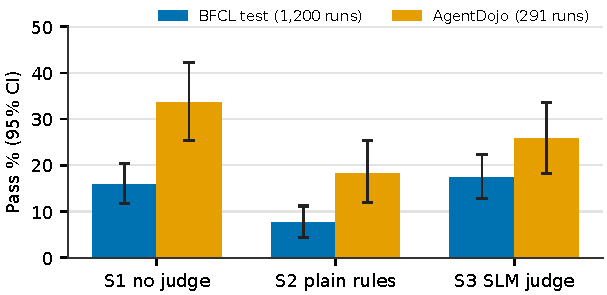
\includegraphics[width=0.6\linewidth]{figs/fig3_test_baselines.pdf}
\caption{Pass rates on BFCL test and AgentDojo (Qwen3 8B agent), 95\% confidence intervals.}\label{fig:test}
\end{figure}

Rules hurt, because they block good calls. Laya as is blocked 87.6\% of judged steps and Granite Guardian called all 169 calls it saw risky, so every run hit the step cap. The SLM judge is the only judge that does not hurt on BFCL. Its +1.5 includes zero, at twice the time per task. On AgentDojo it loses 7.9 points [$-$13.1, $-$3.1], so no judge difference outside BFCL is established.

\subsection{Off the shelf judges, offline}\label{sec:offline}
\begin{table}[H]
\centering\tablestyle
\caption{Primary score (mean F1 of off track and false claim) on the 1,772 validation steps of the 9B agent, guide v1 labels.}\label{tab:offline}
\begin{tabularx}{\linewidth}{Yccc}
\toprule
\textbf{Judge} & \textbf{vs oracle} & \textbf{vs Annotator A} & \textbf{vs Annotator B} \\
\midrule
Plain rules & 0.07 & 0.10 & 0.11 \\
Laya as is & 0.11 & 0.21 & 0.16 \\
Kev 0.8B & 0.15 & 0.12 & 0.07 \\
LettuceDetect (false claim only) & 0.18 & 0.22 & 0.15 \\
\bottomrule
\end{tabularx}
\end{table}
All intervals overlap, so none is reliably ahead. Laya as is stays at AUROC 0.39 to 0.67 across 4 state formats and 8 question wordings. It cuts the end of its input, so on long states it never sees the step it judges, and moving the step first added no signal. Only the hosted Jev classifier showed signal, on closing messages (AUROC 0.81). Off the shelf use is not enough, so Laya is finetuned.

\section{Results: finetuned Laya}\label{sec:laya}
Both heads are fully finetuned with balanced class weights on one RTX 6000 Ada (step head 16 minutes, done head 5 minutes). The step head trains on 8,847 calls (408 bad) and the done head on 3,341 turn ends. The step head's threshold comes from held out dev scenarios. The done head's, 0.56, comes from grouped cross validation on train (Section~\ref{sec:ablations}).

\begin{figure}[H]
\centering
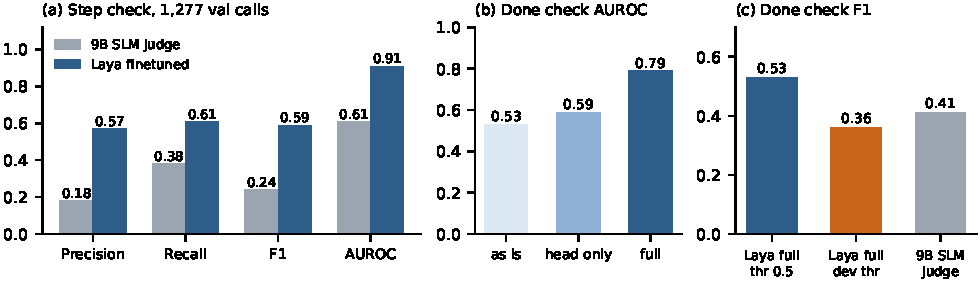
\includegraphics[width=\linewidth]{figs/fig_offline.pdf}
\caption{Finetuned Laya on validation. (a) Replay step labels; the SLM judge used the annotator prompt and 83 of its 1,277 answers did not parse and count as not flagged. (b, c) Done check on 495 turn ends against the oracle, positive class not done; panel (c) shows Laya full at threshold 0.5, at 0.56 from cross validation on train, and at its dev threshold. 20 of the 9B's 495 done check answers did not parse.}\label{fig:offlinelaya}
\end{figure}

\textbf{Step check.} On the 2,427 pooled validation calls the finetuned AUROC is 0.90 against 0.57 as is. It also beats the rule ``flag every irreversible call'' on irreversible calls only (0.74 against 0.50) and on reads only (0.95 against 0.50), so it is not only reading function names. The labels are the replay rules, not yet checked by people. Figure~\ref{fig:offlinelaya}a shows one run. Three reruns on Ada with the same labels (fp16, 3 seeds) give AUROC 0.87 $\pm$ 0.01 and F1 0.47 $\pm$ 0.07 on the same 1,277 calls.

\textbf{Done check.} The full finetune is the only variant with a clear AUROC gain. Its F1 falls from 0.53 to 0.36 when the threshold is the one chosen on dev (0.98, from 50 positives), below the SLM judge's 0.41. A threshold chosen by grouped cross validation on train, without using validation, is 0.56 and gives 0.53, the same as 0.5. The drop came from the small dev split, not the head.

\textbf{Fairer step comparison.} With the SLM judge on its harness prompt and the LLM annotators' labels, Laya's lead on off track tool calls is +8.2 [$-$1.0, +13.5] with Annotator A, +7.2 [$-$3.0, +12.8] with B and +9.2 [$-$0.6, +15.2] where both agree. The harness prompt raised the 9B's call F1 from 0.28 to 0.34, which cut the lead from +14.5 to +8.2 against A. Over the three Ada seeds the mean off track F1 (0.41 / 0.35 / 0.39) is close to this run, but one seed scores 0.17 to 0.22, below the judge's 0.29 to 0.34, so the lead is within seed noise. The 9B judge writes about 1,500 output tokens per call and 2,380 per closing message. Laya runs one forward pass of a 0.4B encoder.

\subsection{Live on the agent}
\begin{table}[H]
\centering\tablestyle
\caption{Live results, 120 validation tasks, Qwen3.5 9B agent. Intervals are paired bootstrap over 15 scenarios.}\label{tab:live}
\begin{tabularx}{\linewidth}{Yrlrr}
\toprule
\textbf{System} & \textbf{Pass} & \textbf{vs no judge [95\% CI]} & \textbf{Judge tok.} & \textbf{s / task} \\
\midrule
No judge & 43.3\% & & 0 & 207 \\
Done check, Laya & 45.8\% & +2.5 [$-$5.0, +10.8] & about 0 & 234 \\
Done check, 9B SLM judge & 43.3\% & +0.0 [$-$5.8, +7.5] & 10,334 & 454 \\
Done check, oracle & 46.7\% & +3.3 [$-$5.0, +12.5] & 0 & 235 \\
Step and done checks, Laya & 42.5\% & $-$0.8 [$-$7.5, +6.7] & about 0 & \\
Step and done checks, 9B SLM judge & 44.2\% & +0.8 [$-$5.0, +7.5] & & \\
Step and done checks, oracle & 47.5\% & +4.2 [$-$1.7, +10.8] & 0 & \\
\bottomrule
\end{tabularx}
\end{table}
No live difference is significant. Two identical no judge runs disagree on 28 of 120 tasks. This agent leaves little room, since a perfect checker adds only +4.2 against +9.2 on the weaker 4B agent. The Laya done check is 2.5 points above the SLM judge done check at about zero judge tokens and half the time per task, which is not significant. A first run gated every closing message with the done head and scored 37.5\%. It was a bug in our wiring and is fixed.

\subsection{Primary metric on validation}
\begin{table}[H]
\centering\tablestyle
\caption{Finetuned Laya against the 9B SLM judge on the 1,772 validation steps, scored against the guide v2 LLM labels. Paired bootstrap over scenarios. The proposal's scoring counts Laya's ``not done'' as a false claim. The 9B used its harness prompt; 33 of its answers (1.9\%) stayed unparsed and count as not flagged.}\label{tab:primary}
\begin{tabularx}{\linewidth}{P{0.12\linewidth}YYYY}
\toprule
\textbf{Labels} & \textbf{Off track, all steps} (Laya / 9B) & \textbf{False claim} (Laya / 9B, positives) & \textbf{Primary,} Laya $-$ 9B & \textbf{Off track, tool calls,} Laya $-$ 9B \\
\midrule
Annotator A & 0.30 / 0.34 & 0.07 / 0.05 (15) & $-$1.0 [$-$7.3, +3.2] & +8.2 [$-$1.0, +13.5] \\
Annotator B & 0.27 / 0.29 & 0.10 / 0.05 (10) & +2.0 [$-$5.4, +7.1] & +7.2 [$-$3.0, +12.8] \\
Both agree & 0.30 / 0.31 & 0.07 / 0.06 (6) & +0.5 [$-$6.7, +5.1] & +9.2 [$-$0.6, +15.2] \\
\bottomrule
\end{tabularx}
\end{table}
The primary hypothesis is not met on validation and not yet tested. Over all steps Laya trails the 9B slightly on off track, because its done head only signals false claims. It leads on tool calls by 7 to 9 points in this run, less than the spread between seeds. False claim is near zero for both on 6 to 15 positives, and Laya has no false claim head yet.

\section{Ablations}\label{sec:ablations}
\begin{figure}[H]
\centering
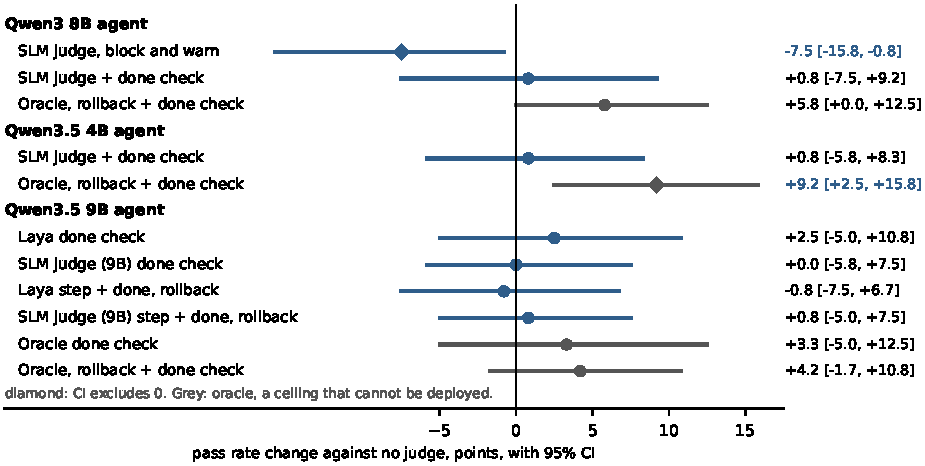
\includegraphics[width=0.95\linewidth]{figs/fig_forest.pdf}
\caption{Pass rate change against no judge on validation (120 tasks per system). Qwen3 8B and 4B rows are from the correction action study, the 9B rows from the live runs.}\label{fig:forest}
\end{figure}

\begin{table}[H]
\centering\tablestyle
\caption{Ablations run so far.}\label{tab:ablations}
\begin{tabularx}{\linewidth}{P{0.2\linewidth}Y}
\toprule
\textbf{Ablation} & \textbf{Result} \\
\midrule
Correction action (Qwen3 8B) & Block and warn does not help even with the oracle (+2.5 [$-$1.7, +6.7]) and hurts with the SLM judge (18.3\% against 25.8\%). Rollback removes that damage (22.5 to 24.2\%). A vote of 3 does not help (20.8\%, $-$5.0 [$-$12.5, +1.7]). Rollback plus the done check with the oracle: +9.2 [+2.5, +15.8] on Qwen3.5 4B and +5.8 [0.0, +12.5] on Qwen3 8B. No deployable judge has moved results. \\
Laya head only against full finetune & Done check AUROC 0.53 as is, 0.59 head only, 0.79 full. Step check AUROC 0.57 as is, 0.90 finetuned. \\
Laya against plain rules, same v2 labels (A / B) & Primary F1 0.07 / 0.06 for rules, 0.18 / 0.19 for Laya. Off track on tool calls 0.16 / 0.14 against 0.42 / 0.36. False claim 0.00 / 0.00 against 0.07 / 0.10, no paired interval yet. The rules flag 299 calls at precision 0.08 to 0.09. On made up values, which Laya does not output, the rules score 0.44 / 0.52. \\
SLM judge prompt & Harness prompt instead of the annotator prompt: 9B call F1 0.28 to 0.34 (against A). \\
Agent reasoning & On is 36.7\% against 43.3\% off, and 2.5 times slower. \\
Annotation guide version & Kappa against the human check on the fresh sample: A 0.71 (v2) to 0.84 (v3), B 0.66 to 0.71. The fresh sample's consensus was labelled under the first v3 draft, so the rise partly reflects v3's own rules. False claim agreement fell under v3 (Section~\ref{sec:annot}). \\
Done head use & As a gate on every closing message 37.5\%, as a done check only 42.5\%. \\
\bottomrule
\end{tabularx}
\end{table}

\begin{table}[H]
\centering\tablestyle
\caption{Phase 3 reruns on Ada (RTX 2080 Ti, fp16), 31 October. Step head: mean $\pm$ sd over 3 seeds on the 1,277 calls of the 9B validation run, AUROC against the replay labels, off track F1 against the v2 annotators (A / B / both agree). Done head: the 495 validation turn ends. Write up: \code{analysis/2026-10-31\_step\_nobt\_and\_done\_cv.md}.}\label{tab:phase3}
\begin{tabularx}{\linewidth}{P{0.3\linewidth}Y}
\toprule
\textbf{Rerun} & \textbf{Result} \\
\midrule
Step head, original labels & AUROC 0.87 $\pm$ 0.01 (0.91 in the run of Figure~\ref{fig:offlinelaya}). Off track F1 0.41 / 0.35 / 0.39, but single seeds range from 0.17 to 0.53. \\
Step head without ``breaks task'' (209 instead of 408 bad training calls) & Off track F1 0.41 / 0.35 / 0.37: agreement with the annotators is unchanged, so the original labels are kept. AUROC 0.79 $\pm$ 0.03 is against labels that still include the rule. \\
Done head threshold from 5 scenario grouped folds of train & 0.56, chosen without validation: F1 0.53 (precision 0.55, recall 0.51), the same as at 0.5. The dev threshold of 0.98 gives 0.36. Thresholds of single folds range from 0.17 to 0.87, so one small split cannot be trusted. \\
\bottomrule
\end{tabularx}
\end{table}

\textbf{Planned.} Drop the plan, recent calls or evidence list from Laya's input and measure off track detection. Three seeds for every remaining finetune, reported as mean $\pm$ sd. The escalation budget (0, 10, 20, 30 and 100\% of uncertain steps to the SLM judge) is a stretch item.

\section{Annotation quality check}\label{sec:annot}
Swayam and Aaditya each labelled every sampled step blind, and Pavan refereed their disagreements. They saw neither the LLM labels nor the oracle labels. The sample is two rounds of 100 validation steps, half flagged by the annotators, with kappa reweighted to the real mix. The proposal's rule: below 0.6 rewrite the guide, from 0.6 to 0.8 label more steps. The bar is 0.7.

\begin{figure}[H]
\centering
\begin{minipage}[c]{0.43\linewidth}
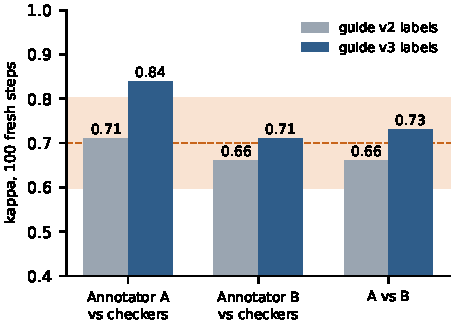
\includegraphics[width=\linewidth]{figs/fig_kappa.pdf}
\end{minipage}\hfill
\begin{minipage}[c]{0.55\linewidth}
\captionof{figure}{LLM annotators against the human consensus on the fresh sample, kappa reweighted. The shaded band is the proposal's ``label more steps'' range, the dashed line the 0.7 bar. Guide v3 was written from the pilot, so the fresh sample is the fair test.}\label{fig:agreement}
\end{minipage}
\end{figure}

\begin{table}[H]
\centering\tablestyle
\caption{Kappa against the consensus (reweighted, problem against fine). $^{*}$The fresh sample's consensus was labelled under the first v3 draft.}\label{tab:agreement}
\begin{tabularx}{\linewidth}{Ycccc P{0.25\linewidth}}
\toprule
\textbf{Round} & \textbf{Checkers} & \textbf{vs A} & \textbf{vs B} & \textbf{A vs B} & \textbf{Decision} \\
\midrule
Pilot, guide v2 & 0.89 & 0.42 & 0.60 & 0.66 & rewrite the guide \\
Fresh sample, guide v2$^{*}$ & 0.87 & 0.71 & 0.66 & 0.66 & label more steps \\
Fresh sample, guide v3 & 0.87 & 0.84 & 0.71 & 0.73 & label more steps \\
All 200 steps, guide v3 & & 0.87 & 0.71 & 0.76 & optimistic, includes the pilot \\
\bottomrule
\end{tabularx}
\end{table}
Checker against checker is computed on the raw sheets before refereeing. The weaker annotator, B, is at 0.71 (0.69 unweighted), in the ``label more steps'' band, so the next 100 check steps come from the test runs. The v2 labels on all validation steps have not been redone with v3. The checkers labelled the fresh sample from the first v3 draft. Two rules were reversed afterwards and no fresh sample label depends on them. On 7 contested pilot steps Shuban's blind second pass sided with the annotators every time, which would lift the pilot kappas from 0.42 and 0.60 to 0.57 and 0.78. The rule that a name the agent chose itself needs asking is kept but contested. The weakest class is false claims at turn ends (kappa 0.38 to 0.46 on a handful of positives), and false claims are half of the primary metric. Guide v3 lowered false claim agreement on the fresh sample (A 0.76 to 0.46, B 0.49 to 0.38; on the pilot B is at 0.00), while turn end done against not done rose (A 0.66 to 0.78, B 0.56 to 0.61). The next guide revision targets false claims.

\section{Challenges and mitigation}\label{sec:challenges}
\begin{table}[H]
\centering\tablestyle
\begin{tabularx}{\linewidth}{P{0.4\linewidth}Y}
\toprule
\textbf{Challenge} & \textbf{Mitigation} \\
\midrule
False claims are rare: 6 to 15 on validation by the LLM labels, while the primary metric needs about 300. Laya has no false claim head. & Test passes until 300 false claims or 8 passes, rule fixed before seeing test results. A typed closing message head. \\
The oracle's off track label disagrees with the annotators (kappa 0.04 to 0.15) yet is set on 276 of the step head's 408 bad training calls. & Retrained without it (3 seeds): agreement with the annotators is unchanged, so the labels are kept (Table~\ref{tab:phase3}). Step check results are still scored against labels that include it. \\
Annotators disagreed on turn ends (kappa 0.54 under guide v1, 0.61 under v2). Under v3 they still agree with each other at only 0.61 to 0.62, and B with the check at 0.60 to 0.61. & 200 step human check, guide v3. Next: 100 more check steps from test, a third annotator for closing messages if false claim agreement stays low. \\
Dev threshold on 50 positives overfit the done head (F1 0.36 against 0.53 at 0.5). & Threshold from grouped cross validation on train: 0.56, F1 0.53 on validation. The dev threshold is dropped. \\
The step head's off track F1 ranges from 0.17 to 0.53 over 3 seeds, wider than its lead over the SLM judge. & Every finetune reported as mean $\pm$ sd over 3 seeds. The test claim rests on the paired bootstrap and the seed spread. \\
Little room on the 9B agent and a noisy pass rate (oracle +4.2, 28 of 120 tasks flip between identical runs). & Three seeds, the larger test set, paired bootstrap. Online pilot on the 4B agent if time allows. \\
Compute: Ada 2080 Ti cards are slow and lack fast bf16, and directed runs with a 27B model would cost too many GPU hours. & 9B runs on a 48 GB card on Turing, fp16 jobs on Ada, Granite on CPU. Directed runs dropped by team decision (24 October), so unneeded irreversible calls and made up values stay below Gate 1 and are pooled into one bad step class. \\
BFCL quality: unsound keys, and the turn where the agent should ask is never scored. & Cleaned split, empty turn check, act or ask decision accuracy reported if time allows. \\
\bottomrule
\end{tabularx}
\end{table}

\section{Changes from the proposal}\label{sec:changes}
This report is measured against the revised proposal of 24 October. Changes since then: directed runs with Qwen3.8 27B dropped, so the step head trains on pooled natural mistakes of Qwen3.5 9B and Qwen3 8B. Test baselines ran with the Qwen3 8B agent and judge and are to be rerun with the 9B. Test passes go up to 8, stopping at 300 false claims. The planned 350 step check of each automatic label rule was not run as specified; retraining the step head without the failed oracle rule did not change agreement with the annotators. Block and warn became rollback plus the done check, which adds a done head at turn end. The heads are binary: Q3 is folded into the step head and Q1 and Q2 are not yet separate outputs, so the per question comparison is still to come. GLM 5.3 Flash is used in place of GLM 5.3. From proposal v5 to the revision: the agent changed from Qwen3 8B to Qwen3.5 9B, hand labelling of test steps became two LLM annotators with a 200 step human check, and Gemma 4 12B replaced Qwen3 14B as the reference judge.

\section{Timeline to the final submission}\label{sec:timeline}
Final submission is 15 November, evaluations 16 to 19 November. The critical path is test passes, test annotation, human check, then the primary metric on test.

\begin{figure}[H]
\centering
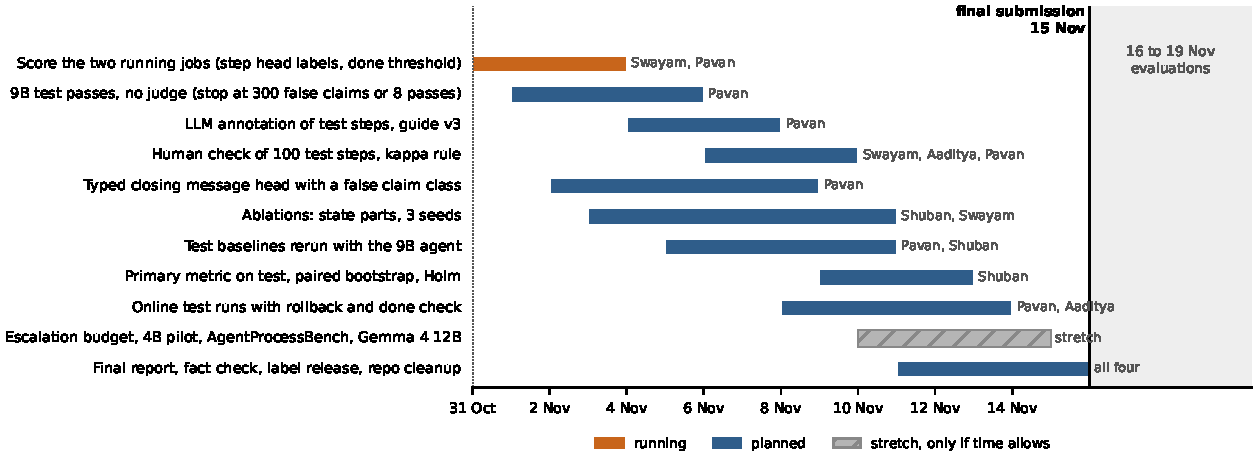
\includegraphics[width=\linewidth]{figs/fig_timeline.pdf}
\caption{Plan to 15 November. Hatched bars are stretch items that are dropped first.}\label{fig:timeline}
\end{figure}

\begin{table}[H]
\centering\tablestyle
\caption{Work plan.}\label{tab:timeline}
\begin{tabularx}{\linewidth}{P{0.14\linewidth}YP{0.2\linewidth}}
\toprule
\textbf{Dates} & \textbf{Work} & \textbf{Owner} \\
\midrule
31 Oct to 3 Nov & Phase 3 reruns on Ada scored and merged (done 31 Oct). Step head seeds under the final settings. & Swayam \\
1 to 7 Nov & 9B test passes without a judge, 4 first and up to 8 if short of false claims. LLM annotation of the test steps with guide v3. & Pavan \\
2 to 9 Nov & Typed closing message head with a false claim class, frozen before test. Human check of 100 test steps, Pavan refereeing. & Pavan; Swayam, Aaditya \\
3 to 10 Nov & State part ablation, 3 seeds. Rerun of the test baselines with the 9B. & Shuban, Swayam, Pavan \\
9 to 13 Nov & Primary metric on test, paired bootstrap, Holm correction. Online test runs with rollback and done check, one pass per system. & Shuban; Pavan, Aaditya \\
11 to 15 Nov & Final report, fact check, release of the checked labels, repository clean up. & All four \\
Stretch & Escalation budget, 4B online pilot, AgentProcessBench and AgentHallu, Gemma 4 12B reference, v3 relabel of all validation steps. & Dropped first \\
\bottomrule
\end{tabularx}
\end{table}
If the test passes slip past 5 November, the online runs and the ablations are cut before the primary metric is.

\section{Repository}\label{sec:repo}
\url{https://github.com/ch-pavan/lma-grp-project} holds all code, data and results. Key folders: \code{shuban\_findings/} (harness, baselines, correction modes, off the shelf judges), \code{analysis/} (oracle and step labels, annotation, Laya finetuning and evaluation, write ups), \code{human\_check/} (guides, samples, sheets, results), \code{runs/} (run outputs, labels, Laya datasets, job scripts), and \code{docs/phase\_plan.md} (plan with owners). GPU job scripts are in \code{runs/turing/} and \code{runs/ada/}.

\begin{tabular}{@{}l@{}}
\code{sh runs/unpack\_data.sh}\quad rebuild \code{runs/data} from the repository\\
\code{python analysis/primary\_val.py}\quad primary metric on validation\\
\code{python human\_check/score.py human\_check/val2 -{}-guide v3}\quad annotation check\\
\code{python analysis/score\_step\_variants.py runs/data/laya\_runs/ada\_step\_nobt}\quad Table~\ref{tab:phase3}, step head\\
\code{python analysis/done\_threshold\_cv.py runs/data/laya\_runs/ada\_done\_cv}\quad Table~\ref{tab:phase3}, done threshold
\end{tabular}

\end{document}
